\chapter[CIAC]{CIAC}
Este capítulo traz a proposta para o sistema anti-colisão, titulado de CIAC.
Será descrito e justificado sobre os equipamentos a serem utilizados, o funcionamento
do sistema e a exemplificação de cenários de uso do sistema.

\section{Componentes Utilizados}

Vários sensores e componentes eletrônicos serão utilizados para o desenvolvimento
do sistema. Eles são importantes para possibilitarem: comunicação entre
os centros de processamentos de cada automóvel; visualização do estado presente
quando em funcionamento; emissão de alertas para o condutor do veículo; detecção
de inteção de ultrapassagem e análise de posição do veículo.

\subsection{TRANSPONDER VDL 4000/VTE CNS SYSTEMS}

\subsubsection{Conceito}
Transponder é a abreviatura para transmiter/responder, ou seja, um sistema
composto de um leitor, que solicita os dados armazenados em um segundo
transmissor, ou seja, um sistema de comunicação em duas vias.

Existem transponders passivos e ativos:

\begin{itemize}
  \item Passivos: Transponders passivos são frequentemente encontrados,
  sendo equipamentos relativamente simples, podendo ser observados na forma
  de etiquetas ou chips, desprovidos de baterias ou fontes próprias de energia
  , são energizados e ativados quando na presença do leitor, por meio da
   emissão de radiofrequência. Frequentemente utilizados no meio
   comercial/industrial, bem como em chaves codificadas.
  \item Ativos: Transponders ativos são em geral mais complexos que os
  modelos passivos, pois envolvem a emissão de dados via radiofrequência
  tanto na requisição de dados bem como no envio da resposta. Com aplicação
  difundida nos campos aeronáutico e naval, servem como base de
  comunicações/identificação a longa distância. Por serem equipamentos ativos,
  necessitam de uma fonte energética constante. Possuem uma taxa de
  transmissão de dados muito superior aos modelos passivos.
\end{itemize}

Para aplicação em nosso caso, abordaremos apenas o conceito de transponders ativos.

\subsection{Como Funciona?}
Um transponder ativo funciona à base de emissão de radiofrequência, tanto para
solicitar os dados de outros dispositivos bem como para emitir os dados
armazenados em si. Desta forma, é necessário notar que um transponder não
fornece dados, sejam eles quaisquer sejam, mas se apresenta como uma solução
versátil para comunicação à longa distância, transmitindo dados
armazenados/coletados pelo sistema ao qual está acoplado.

No caso da aplicação aeronáutica, os transponders são utilizados para
transmitir às estações de controle em solo dados como posição, altitude,
velocidade e direção das aeronaves, sendo que esses dados são obtidos
por diferentes sensores.

Como referência, já existe um sistema de transponders homologado
para identificação veicular em rodovias no Brasil, o SINIAV, que
tem o intuito de identificar os veículos que trafegam pelas
rodovias ao passarem por postos de controle espalhados ao longo do
trajeto. Uma aplicação mais rotineira de uma espécie de transponder
é o sistema de pagamento automático de pedágios em estradas sob concessão.

\subsubsection{Aplicação no caso}
Para o caso ao que esta pesquisa se aplica, o modelo de transponder seria
utilizado para transferir entre os veículos os dados obtidos, ou seja,
velocidade e posição, que serão respectivamente coletados pelo velocímetro
e GPS. Desta forma, conseguimos que esses dados, necessários aos cálculos
base do sistema, sejam transmitidos à distância necessária e com alto grau
de confiabilidade, uma vez que, ao utilizar radiação eletromagnética para
transmitir os dados, um transponder não sofre com interferências climáticas,
ambientais e demais, o que o torna uma boa opção para integrar um sistema crítico.

\subsubsection{Modelo escolhido}
Para integrar o projeto, foi escolhido um sistema já desenvolvido para aplicação
veicular, visando tráfego de equipes de solo em aeroportos, sendo ele o seguinte:

CNS Systems – VDL4000/VTE \cite{datasheet_transponder}
O modelo aqui referenciado apresenta compatibilidade de conexão com os demais
componentes via porta RS422. O alcance de um transmissor VHF é delimitado pela
 linha de visão (line of sight), sendo que esta pode ser calculada da seguinte
 forma:

 $ D = \sqrt{12.7 \times A_{m}} $

 Onde D é o referido alcance, e Am é a altura a que o receptor se encontra
 localizado. No caso, o veículo referência possui uma altura de 1464mm, ou
 1,464 metros, ou seja, o alcance com o transmissor posicionado no teto do
 veículo seria de aproximadamente 4,3 Km em terreno plano, mostrando-se
 adequado à aplicação no caso proposto.

 É importante notar que a frequência utilizada é regulamentada pela ANATEL
 (Agência Nacional de Telecomunicações) para transmissão em solo, não havendo
  assim restrições em relação à radiopropagação ou níveis de energia
  eletromagnética.

\subsection{Escolha Sistema de Posicionamento Global}

Para a escolha do GPS foram analisados vários dispositivos disponíveis no mercado
e assim foi justificada de acordo com alguns parâmetros. A pesquisa completa está
ilustrada no Apêncide \ref{appendix:escolha_gps}.

\subsubsection{Especificações do GPS}

O GPS possui dois modos de operação, o padrão, Standard Positioning Service,
SPS, e o preciso, Precise Positioning Service, PPS. O SPS é gratuito e tem
precisão de 120 a 140 m e de 10 a 20 m, enquanto o PPS, é de uso restrito
militar e apresenta precisão de 10 a 20 m. O SPS tem precisão limitada e
seletiva imposta pelo Departamento de Defesa Americano, por um processo de
criptografia aplicado em um dos códigos do sistema que torna as medições
menos precisas se necessário \cite{6gps}.

Os satélites transmitem continuamente um sinal de rádio com informações sobre
a sua posição orbital e tempo marcado por seu relógio atômico interno \cite{7gps}.
 Esse sinal eletromagnético é chamado de onda portadora e passa por um
 procedimento de modulação antes de ser irradiado pelo espaço, esse processo
 de modulação consiste em modificar um sinal eletromagnético de forma que
 transporte informações, como dados de posição e tempo \cite{8gps}.

O sistema receptor armazena o tempo medido e os valores de tempo registrados
pelos satélites no momento do envio da onda portadora, com base nesse dado e
 na velocidade de propagação das ondas, que é conhecida, através da equação
 a seguir se obtém a distância \cite{8gps}.

 $ \Delta S = V \times  \Delta t $

 Onde:

 $ \Delta S $ é a distância entre o satélite e o receptor.
V é a velocidade de propagação da onda.

$ \Delta t $ é o tempo de envio da onda portadora.

Como citado na seção 1.1, o GPS possui três segmentos, espacial, de controle e
de usuário, a figura \ref{fig:segmentos_gps} ilustra a iteração dos segmentos.


\begin{figure}[h]
  \centering
  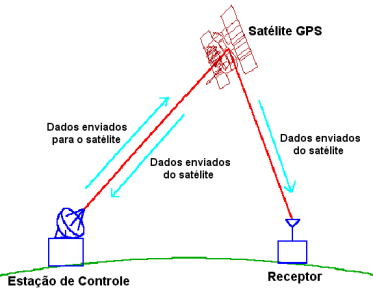
\includegraphics[width=250px, scale=1]{figuras/segmentos_gps}
  \caption{Segmentos de GPS  \cite{9gps}}
\label{fig:segmentos_gps}
\end{figure}


\subsubsection{Justificativa da Escolha}

  \subsubsubsection{ME-1000RW}

  O ME-1000RW é um módulo receptor GPS com antena acoplada. A antena é conectada
  ao receptor através de um Amplificador de Baixo Ruído. O receptor é capaz de
  receber sinais de até 65 satélites GPS e informar a posição e o tempo precisos,
  além disso possui baixo consumo \cite{11gps}. A figura \ref{fig:gps_me1000} e a tabela
  \ref{table:especificacao_gps_me1000}
  descrevem as  características do produto. O preço desse modulo é de R\$ 98,99 \cite{12gps}.


\begin{table}[ht]
\caption{Especificações do ME-1000RW Baseado em: \cite{11gps}}
\centering
\begin{tabular}{| l |  p{5cm} |}
\hline
Característica & Valores \\
\hline
Canais & 65 \\
\hline
Frequência & 1575,42 MHz \\
\hline
Precisão de distância & 5 m \\
\hline
Precisão de tempo & 300 ns \\
\hline
Precisão de velocidade & 0,1 m/s \\
\hline
Limite de operação para velocidade & 515 m/s \\
\hline
Peso & 28 g \\
\hline
Dimensões L x A x P & 32 x 32 x 8 mm \\
\hline
Tensão de operação & 3,6 a 6 VDC \\
\hline
Corrente máxima & 23 mA \\
\hline
Temperatura de operação & - 20ºC a +60ºC \\
\hline
Temperatura de armazenamento & -40ºC a +80ºC \\
\hline
Sensibilidade & -161 dB \\
\hline
\end{tabular}
\label{table:especificacao_gps_me1000}
\end{table}


\begin{figure}[h]
  \centering
  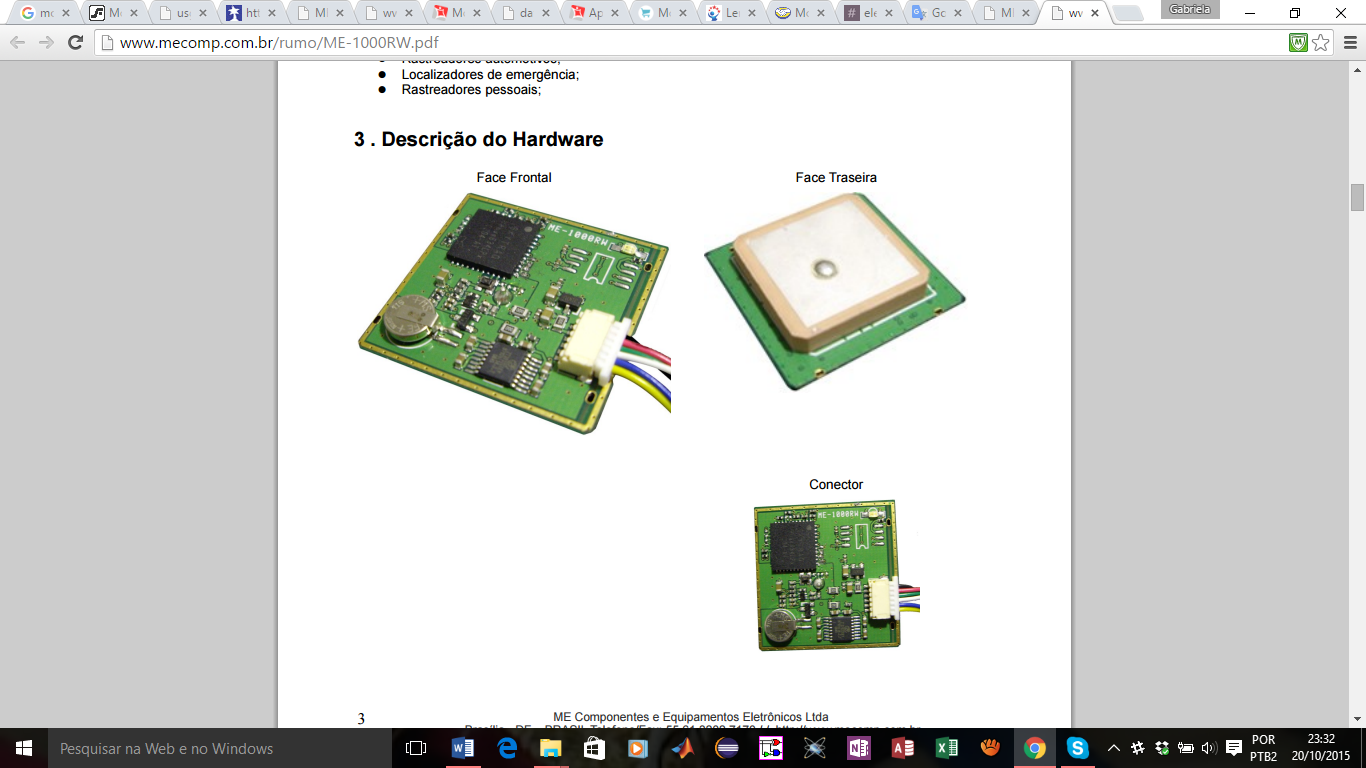
\includegraphics[width=200px, scale=1]{figuras/gps_me1000}
  \caption{ME-1000RW \cite{11gps}}
\label{fig:gps_me1000}
\end{figure}



\subsection{Escolha Lidar}

O Lidar é uma tecnologia de detecção usado para medição de distâncias ou
outras informações relevantes. O Lidar funciona com a emissão de um laser
que será refletido por um objeto (o que se deseja medir a distância) e depois
detectado fazendo uso das propriedades da luz para se obter as informações
desejadas. Seu funcionamento é parecido com o do radar, porém com pulsos de
laser ao invés de ondas de rádio.


\begin{figure}[h]
  \centering
  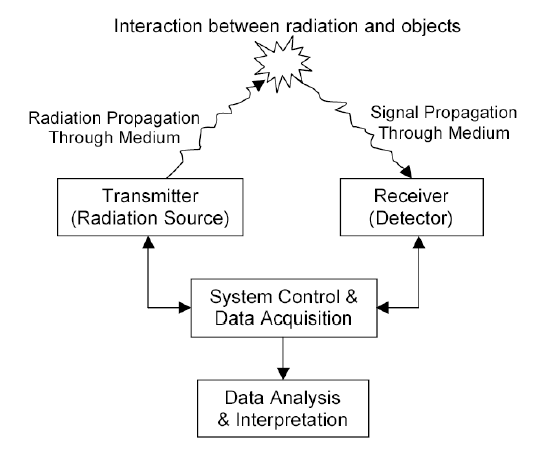
\includegraphics[width=400px, scale=1]{figuras/funcionamento_lidar}
  \caption{Esquemático do funcionamento do Lidar}
\label{fig:funcionamento_lidar}
\end{figure}

\subsubsection{Justificativa da escolha}
O Lidar será utilizado no CIAC para medição de diversas distâncias entre carros,
sendo eles os que estão sendo ultrapassados ou os que estiverem na via oposta
durante a ultrapassagem.

	A detecção de luz e o mapeamento com o Lidar é um método preciso para medição
  de referências espaciais e distâncias de objetos, além de fazer uma varredura
  para obtenção dos dados não sendo um detector pontual. O Lidar servirá como um
  sensor para uma maior confiabilidade do sistema CIAC e permite a obtenção de dados
  a partir de ondas eletromagnéticas (o processo físico é extremamente rápido)
  fazendo com que a demora para obtenção da distância entre um carro e outro
  dependa em sua maior parte apenas do processamento desses dados. Uma grande
  precisão em um pequeno intervalo de tempo faz do Lidar uma boa opção
  na utilização do projeto.

	Uma grande desvantagem do Lidar é que sua utilização não é efetiva em
  climas adversos como chuva e neblina devendo ser utilizado em boas condições
  climáticas, na maioria das aplicações com Lidar as detecções são feitas
  de noite onde seu desempenho costuma ser melhor.

\subsubsection{Especificação Lidar}

O Lidar utilizado será o HDL-64E da Velodyne que possui uma alta definição e
consegue captar uma distância de até 120 m com alta resolução.

Especificações de acordo com a Figura \ref{fig:especificacoes_lidar}

\begin{figure}[h]
  \centering
  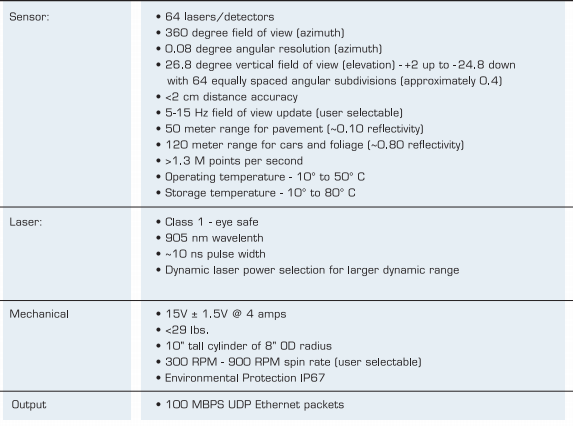
\includegraphics[width=400px, scale=1]{figuras/especificacoes_lidar}
  \caption{Especificações do Lidar}
\label{fig:especificacoes_lidar}
\end{figure}

Design do produto de acordo com a Figura \ref{fig:design_lidar}

\begin{figure}[h]
  \centering
  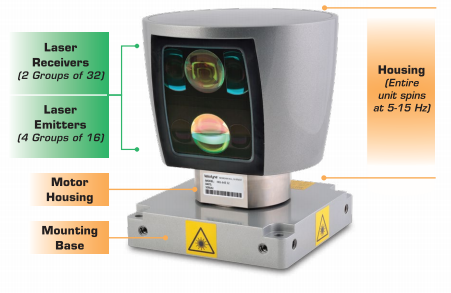
\includegraphics[width=400px, scale=1]{figuras/design_lidar}
  \caption{Design do Lidar}
\label{fig:design_lidar}
\end{figure}


\subsection{Radar}

Um radar mede uma distância, velocidade ou ângulo de objetos através da
utilização de ondas de rádio. O radar emite ondas de rádio que são refletidas
por objetos e depois capta e processa essas ondas refletidas para obtenção das
informações desejadas tendo como base as propriedades das ondas eletromagnéticas.

As principais propriedades dessas ondas são:

\begin{itemize}
  \item A energia normalmente viaja em uma linha reta a uma velocidade constante;
  \item Energia eletromagnética viaja aproximadamente à velocidade da luz;
  \item Essas ondas são refletidas.
\end{itemize}

\begin{figure}[h]
  \centering
  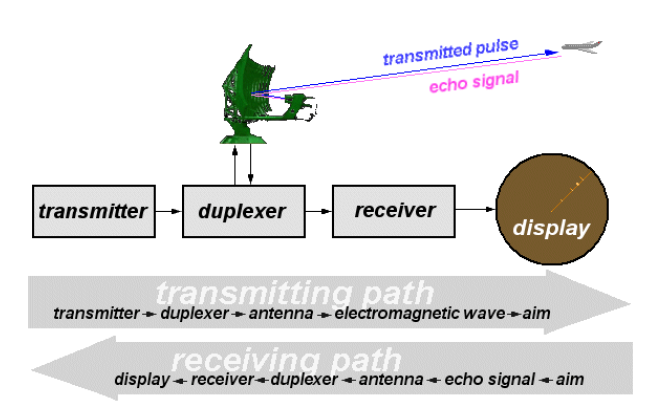
\includegraphics[width=400px, scale=1]{figuras/funcionamento_radar}
  \caption{Esquemático do funcionamento do radar}
\label{fig:funcionamento_radar}
\end{figure}

Os radares funcionam com a emissão de pulsos (transmitted pulses) para posterior detecção dos pulsos refletidos
(echo pulses), isso serve para uma sincronização necessária para a medição de distâncias, já que os pulsos
são emitidos sequencialmente após um período de tempo (PRT) e os pulsos possuem
uma largura determinada.

\begin{figure}[h]
  \centering
  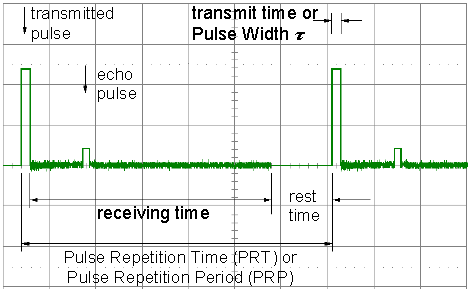
\includegraphics[width=400px, scale=1]{figuras/emissao_pulsos_radar}
  \caption{Gráfico representativo da emissão de pulsos por um radar}
\label{fig:emissao_pulsos_radar}
\end{figure}

A distância entre o radar e o objeto que se quer saber a distância é dada por essa simples equação:

$ R = \displaystyle\frac{Tdelay * C0}{2}$

Onde:

	R: é a distância até o objeto.

	tdelay: é o tempo para o sinal viajar e retornar.

	c0: é a velocidade da luz.

  E as equações para as distâncias máximas e mínimas que um radar pode detectar sem
  causar ambiguidade, sendo trecovery o tempo de recuperação do equipameto
   utilizado, são:


$ Rmax = \frac{(PRT - t) * C0}{2}$

$ Rmin = \frac{(t + Trecovery) * C0}{2}$




Equação teórica do radar:

$p_{r} = \frac{\pi ^{2}p_{t}g^{2}\theta h |K|^{2}l2}{1024ln(2)\lambda ^{2}\gamma ^{2}}$

Onde:

Pt = power transmitted by radar (watts)

Pr = power received back by radar (watts)

g = gain of the antenna (ratio of power on the beam axis to power from an isotropic [i.e.,
radiating equally in all directions] antenna at the same point); it is a measure
of how focused the radar beam is.

$\theta$ = horizontal beamwidth (radians)

$\omega$ = vertical beamwidth (radians)

h = pulselength (m)

|K|2 = dielectric constant for hydrometeors; usually taken as 0.93 for liquid water, 0.197 for
 ice. (Note that for an equivalent mass of frozen precipitation, much less power is returned
 from the ice than from liquid precipitation; thus snow with the same water content is
  less reflective than rain). For this reason, NEXRAD’s clear air mode rather than
  precipitation mode is sometimes used to monitor snow situations because of its greater
  sensitivity).

l = loss factor for attenuation of radar beam, varies between 0 and 1, usually near 1.
 Since the attenuation of the beam is often unknown, it is often ignored.

$\gamma$ = wavelength of radar pulse (m)

r = range or distance to the target (i.e., the distance to an area of precipitation
that reflects the originally transmitted pulse back to the radar).

z = radar reflectivity factor (mm6/m3)

\subsubsection{Justificativa da Escolha}

O radar é um dispositivo amplamente utilizado que possui grande confiabilidade.
Várias empresas automotivas utilizam de radares para detecçao de distâncias e
velocidades já que se pode ter uma medição precisa e as interferências causadas
pelo ambiente ou por condições climáticas poderem, algumas vezes, ser contornados.

\subsubsection{Especificações Radar}

\subsubsubsection{Solução fechada}

Radar ARS-30X da Continental.

Performance pode ser vista na Figura \ref{fig:performace_radar}:
\begin{figure}[h]
  \centering
  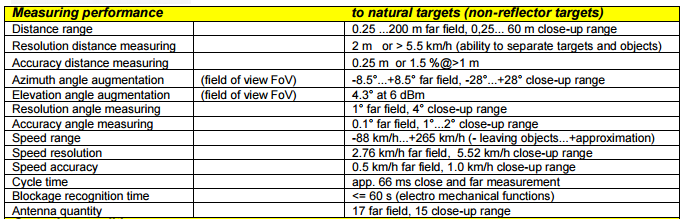
\includegraphics[width=400px, scale=1]{figuras/performace_radar}
  \caption{Performace do Radar ARS}
\label{fig:performace_radar}
\end{figure}

Consumo pode ser vista na Figura \ref{fig:consumo_radar}:
\begin{figure}[h]
  \centering
  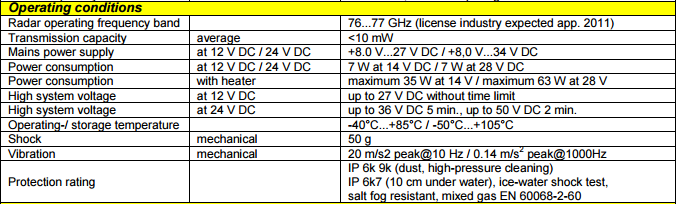
\includegraphics[width=400px, scale=1]{figuras/consumo_radar}
  \caption{Consumo do Radar ARS}
\label{fig:consumo_radar}
\end{figure}

Dimensões pode ser vista na Figura \ref{fig:dimensoes_radar}:
\begin{figure}[h]
  \centering
  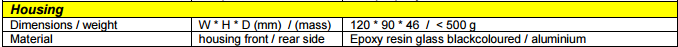
\includegraphics[width=400px, scale=1]{figuras/dimensoes_radar}
  \caption{Dimensões do Radar ARS}
\label{fig:dimensoes_radar}
\end{figure}


\subsubsubsection{Solução Aberta}
Soluções abertas, a serem definidas pelos equipamentos utilizados em sua produção caso se deseje montar um da
Figura \ref{fig:esquematico_radar}.
\begin{figure}[h]
  \centering
  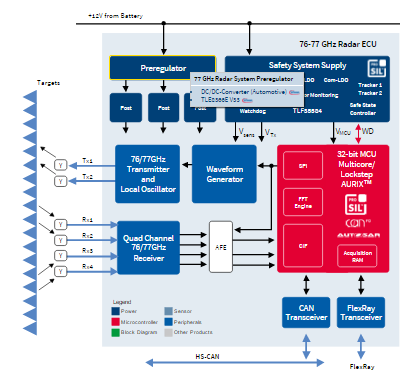
\includegraphics[width=400px, scale=1]{figuras/esquematico_radar}
  \caption{Esquemático dos componentes de um radar}
\label{fig:esquematico_radar}
\end{figure}

\subsection{Baterias Automotivas}

As baterias dos automóveis possuem normalmente essa força eletromotriz de 12 V,
pois são compostas de 6 pilhas ou células de chumbo-ácido. E elas são também
denominadas como baterias de chumbo, porque o seu ânodo (polo negativo) são as
placas de chumbo e o seu cátodo (polo positivo) são as placas de chumbo com óxido
 e chumbo IV ($\mathrm{Pb O_2}$).


Essas baterias possuem altas correntes, que permitem dar partida em motores
 graças aos elevados valores de densidade de potência que apresentam.

Como se observa na figura abaixo, as placas de chumbo revestidas de $\mathrm{Pb O_2}$
(placas negativas) são ligadas ao conector positivo. Enquanto que as placas de chumbo
(placas positivas) são ligadas ao conector negativo. Elas são separadas por algum
papelão, plástico ou algum papel separador microporoso.

Esse conjunto é colocado no compartimento da bateria e mergulhadas em uma solução
aquosa de ácido sulfúrico ($\mathrm{H_2 SO_4}$) com uma densidade de
aproximadamente $1,28 g/cm^{3}$	.

\begin{figure}[h]
  \centering
  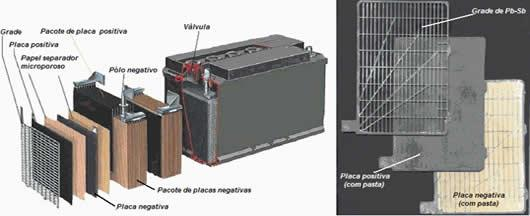
\includegraphics[width=400px, scale=1]{figuras/bateria}
  \caption{Bateria com placa de chumbo}
\end{figure}

As semirreações e a reação global que ocorrem nessa bateria são:\\
Ânodo: $\mathrm{Pb}$ + $\mathrm{HSO_4^{1-}}$ + $\mathrm{H_2 O}$ $\leftrightarrow$
 $\mathrm{PbSO_4}$ + $\mathrm{H_3 O^{1+}}$ + 2e-\\

Cátodo: $\mathrm{Pb O_2}$ + $\mathrm{HSO_4^{1-}}$ + $\mathrm{3 H_3 O^{1+}}$ +
2e- $\leftrightarrow$ $\mathrm{PbSO_4}$ + $\mathrm{5 H_2 O}$\\

\dotfill\\
Reação global: $\mathrm{Pb}$ + $\mathrm{PbO_2}$ + $\mathrm{2HSO_4^{1-}}$ +
$\mathrm{2H_3 O^{1+}}$ $\leftrightarrow$ $\mathrm{2PbSO_4}$ + $\mathrm{4 H_2 O}$

Como pode ser observado pela seta dupla acima, essas reações são reversíveis, o
que significa que é possível recarregar novamente as baterias de chumbo por se
fornecer energia ao sistema, ou seja, é possível passar uma corrente elétrica
-fornecida por um gerador de corrente contínua. Desse modo, o sentido dessas
reações é invertido, ocorrendo a regeneração de grande parte do ácido sulfúrico
e carregando, assim, a bateria. No automóvel, essa diferença de potencial que
fornece energia e recarrega a bateria é feita pelo dínamo ou pelo alternador.

A densidade do ácido sulfúrico ajuda a identificar se a bateria está decarregada.
Visto que sua densidade é 1,28g/cm3; se este valor estiver abaixo de 1,20 g/cm3,
significa que o ácido sulfúrico foi consumido e a bateria está descarregada.
Por isso, essas baterias são muito duráveis.

\input{editaveis/textual/consumo_energetico}

\subsection{Sensor de Rotação}

\subsubsection{Justificativa da escolha}
Para fins de projeto, foi necessário que se escolhessem alguns sensores os quais
possibilitassem que o sistema de alerta anti colisão identificasse quando o motorista
apresenta intenção de ultrapassagem, para esse fim, foi escolhido um sensor de rotação o
 qual identifica a posição angular da direção do veiculo, onde ao girar o volante no
 sentido da ultrapassagem, o mesmo calcula a angulação de giro enviando esses
 dados para o microprocessador, onde será processado todas as ações do sistema.

Segundo a Piher, evidenciado no datasheet do PST-360 \cite{sensor_rotacao}, o referente designer
renovador e único apresenta as seguintes vantagens:

\begin{itemize}
  \item Complementa os atributos do aplicativo de destino;
  \item Integridade mecânica que corresponde ao pedido do cliente pelo design.
  \item O eixo original montou o projeto que monta no ponto de pivô da aplicação;

  \item Sem alavancas , bielas ou interfaces mecânicas necessárias;

  \item Adapta-se a excentricidade do eixo, tolerâncias de montagem e
  desgaste mecânico ao longo da vida da aplicação;

\end{itemize}

O novo PST 360 Piher apresenta uma tecnologia exclusiva sem contato que detecta a posição dos
eixos mais de 360 grau com precisão até +- 0,5\%. Este dispositivo pode ser programado com
saída de escala completa durante ângulos menores. A saída é selecionável entre Analógica ,
PWM e SPI. Além disso, a tecnologia da Piher mantém a sua posição, mesmo depois de uma
interrupção de energia.

Um dos motivos pelo qual o sensor PST-360 foi escolhido é o suporte de encaixe
diretamente no eixo de direção do volante oferecido, de forma que não seja
necessário ter nenhum suporte adicional na sua instalação.

\begin{figure}[h]
  \centering
  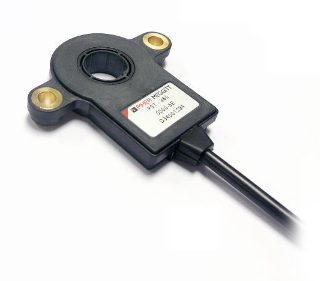
\includegraphics[width=300px, scale=1]{figuras/pst}
  \caption{ Sensor de rotação PST-360}
\label{fig:pst}
\end{figure}

\subsubsection{ESPECIFICAÇÕES DO SENSOR PST-360}

De acordo com o Datasheet \cite{sensor_rotacao} fornecido pelo fabricante Piher, o sensor escolhido
obedece as seguintes especificações:

\begin{itemize}
  \item Linearidade : +- 1\% (0,5\% em cima do pedido );
  \item Projeto magnético simples e robusto;
  \item Faixa Angular: programável de 15º a 360º;
  \item Característica de transferência linear programável (as inclinações positivas e
  uma inclinação negativa podem ser programadas na mesma característica de transferência);

  \item Resolução angular (depende do ângulo elétrico e da velocidade rotatória):
  \item Analógico e PWM: Até 12 bits;
  \item Protocolo de Série (SPI): Até 14 bits;
  \item Diferentes opções de redundância disponíveis;
  \item Características de auto diagnostico;
  \item Vida de rotação: virtualmente ilimitado (dependendo da aplicação e montagem)
  \item Temperatura de funcionamento : de -40ºC a +125ºC;
  \item Sobre a proteção da tensão e a proteção da tensão reversa;
  \item Tensão de alimentação : 5V / 12V / 15V +- 10%
  \item Corrente de alimentação:
  \item 8.5mA para a única versão.
  \item 17mA para a versão redundante.
  \item IP67 (eletrônica);
  \item Cabeamento personalizado e configurações de conector;
\end{itemize}

\subsubsubsection{Exemplos de aplicações}

\begin{itemize}
  \item  Angulo de ponto do pivô que detecta para todas as aplicações;
  \item Fora da estrada/ direção da estrada;
  \item Detecção da posição de pedal;

  \item Máquinas agrícolas, braços de elevadores hidráulicos, colheres, articulações/junções;

  \item Empilhadeiras / manuseio de materiais;

  \item Bombas industriais;

  \item Robótica;

\end{itemize}


\begin{figure}[h]
  \centering
  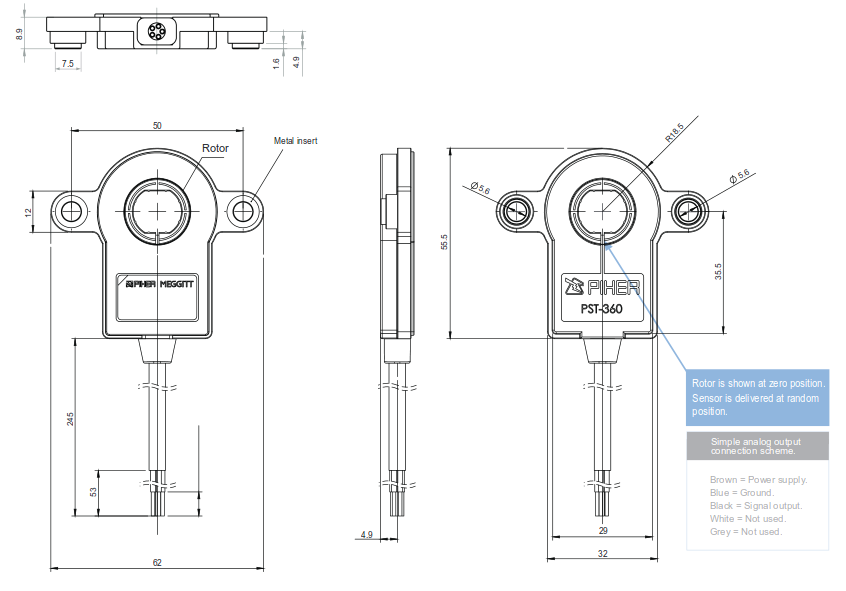
\includegraphics[width=300px, scale=1]{figuras/pst_dimensoes}
  \caption{ Dimensões do PST-360 \cite{sensor_rotacao}}
\label{fig:pst_dimensoes}
\end{figure}

\begin{figure}[h]
  \centering
  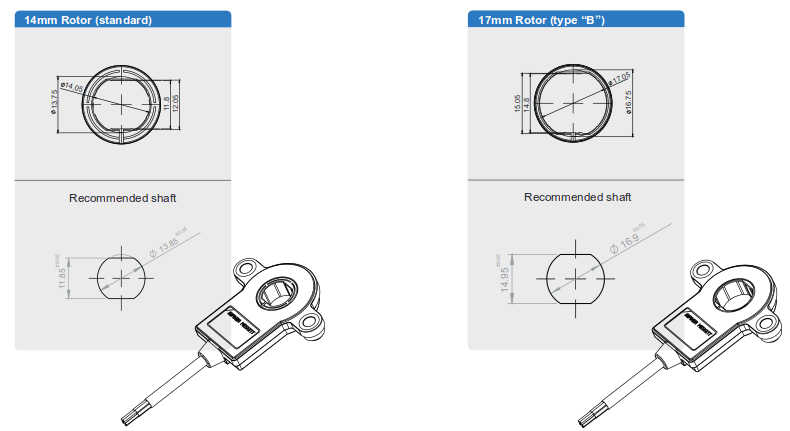
\includegraphics[width=300px, scale=1]{figuras/pst_dimensoes2}
  \caption{ Dimensões do PST-360 \cite{sensor_rotacao}}
\label{fig:pst_dimensoes2}
\end{figure}

\subsubsubsection{Funções de saída padrão}

\begin{figure}[h]
  \centering
  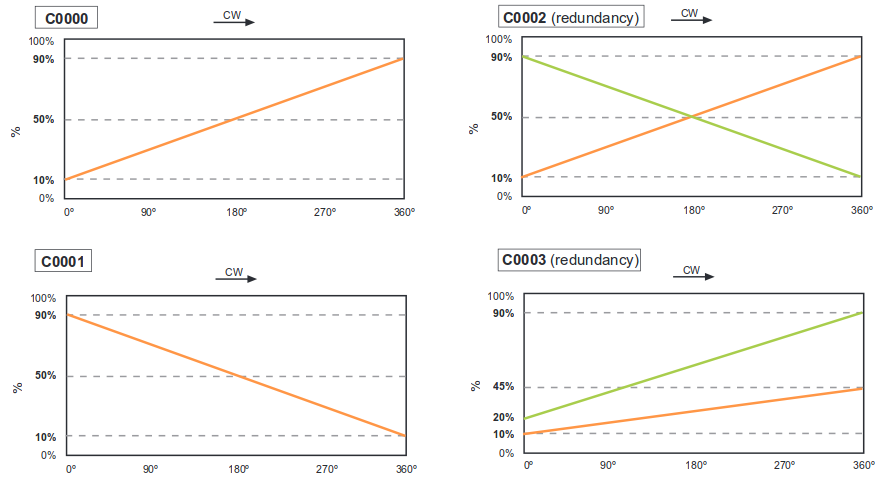
\includegraphics[width=300px, scale=1]{figuras/pst_saida_padrao}
  \caption{ Exemplos de funções padrões geradas pelo PST-360 \cite{sensor_rotacao}}
\label{fig:pst_saida_padrao}
\end{figure}

As partes ferromagnéticas perto do ambiente do sensor, incluindo o eixo,
podem modificar o desempenho do mesmo.



\section{Posicionamento dos Equipamentos}
\subsection{CÂMERA}
A localização da câmera será na região inferior do para-brisa, acima do painel.
Este lugar foi escolhido por não causar prejuízo de visão ao motorista e por ser o mais
indicado para esse tipo de câmera. Esta localização não prejudica o funcionamento do
dispositivo.

\subsection{SENSORES}
Sensores de rotação são implantados no volante. E funcionam conforme a
variação angular. Ao virar o volante, para realizar a ultrapassagem, o sensor calcula o
ângulo e envia os dados para o microprocessador.

\subsection{CAIXA PROTETORA}
Para a alocação da caixa protetora que contém radar, lidar e GPS, é necessário
pensar nas melhores possibilidades levando em conta a temperatura, o espaço e o risco
de choque. Localizações as quais a ergonomia do usuário não seja prejudicada e nem
ofereça riscos danosos ao equipamento.

\subsubsection{PORTA-MALAS}
O espaço do porta malas é uma possibilidade, entretanto, a diminuição de um
espaço tão visado pelos usuários não é indicada. No caso do modelo Gol da
Volkswagem o porta malas contém 285 litros e não deve ser reduzido para que não haja
desapontamento dos compradores.

\subsection{Posicionamento da Caixa}
A caixa protetora contendo o transponder, GPS e o microprocessador, será feita
de Polipropileno, um material bastante versátil que dentre as suas principais
propriedades estão o baixo custo,elevada resistência química e a solventes,
fácil moldagem, alta resistência a fratura por flexão ou fadiga, boa resistência
ao impacto acima de 15 ºC, boa estabilidade térmica.


\begin{figure}[h]
  \centering
  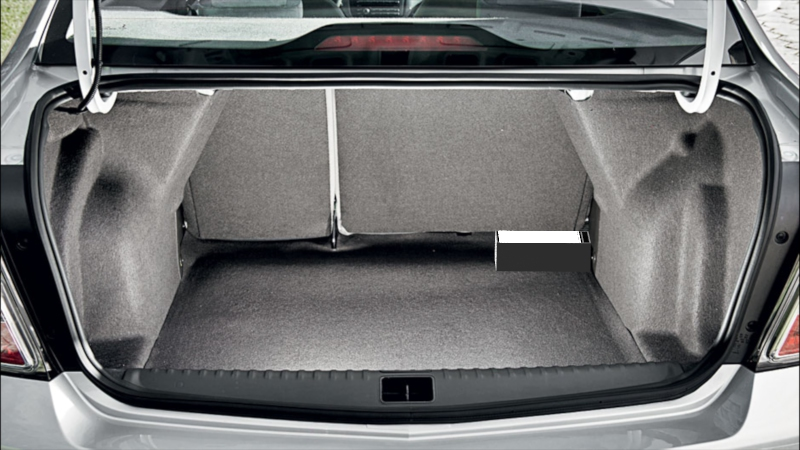
\includegraphics[width=470px, scale=1]{figuras/posicionamento_caixa}
  \caption{Exemplo de alocação da Caixa Protetora no Porta-Malas do veículo}
\label{fig:posicionamento_caixa}
\end{figure}



\section{Funcionamento do Sistema}

O sistema CIAC foi desenhado para funcionar de acordo com o fluxo de uso ilustrado
em linguagem BPM na Figura \ref{fig:funcionamento_sistema}.

\begin{figure}[h]
  \centering
  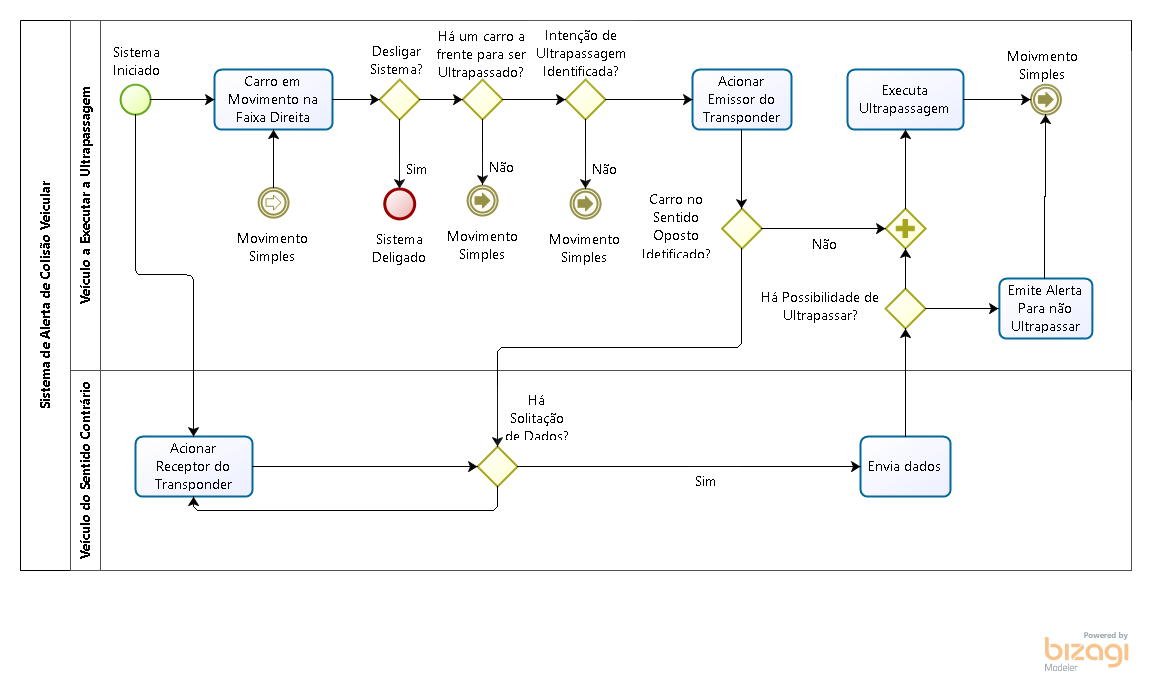
\includegraphics[width=470px, scale=1]{figuras/funcionamento_sistema}
  \caption{Fluxograma de Funcionamento do Sistema CIAC}
\label{fig:funcionamento_sistema}
\end{figure}

O sistema pode se comportar de duas maneiras diferentes nos veículos que possuem
o CIAC instalado: A Executar a Ultrapassagem e No Sentindo Oposto. Cada uma das duas
está representada na sua respectiva lane do fluxo de uso.

\subsection{Veículo a Executar a Ultrapassagem}
O CIAC é iniciado quando é dada a partida no automóvel. Na lane do veículo a ultrapassar,
há um estado de inércia do sistema, representado pelo evento: Carro em Movimento
na Faixa Direita. Este permanece neste estado até que não exista inteção de
ultrapassagem.

Caso seja identificada a intenção de desligar o sistema, esta é realizada, caso
contrário o CIAC volta para o estado de inércia na faixa direita.

O CIAC identifica através do sistema de sensoriamento se há um carro a frente
para ser ultrapassado. Se existir, o fluxo segue para o próximo estágio, caso
contrário, segue o sistema de Movimento Simples.

Identificado o carro para ser ultrapassado a frente, o CIAC verifica se há a
intenção por parte do motorista de ultrapassá-lo. Existindo, o fluxo do sistema
segue a frente. Caso não seja identificada a inteção, o Movimento simples
é tomado.

No momento que a intação de ultrapassagem é identificada, é enviada uma mensagem
pelo transponder em Broadcast para verificar se há um outro veículo em movimento
no sentido oposto. Não havendo, a ultrapassagem segura é executada.

No caso em que há um carro no sentido oposto, uma troca de mensagens é realizada
via transponder e com base nesses dados, são executados cálculos com o intuito
de verificar se existe a possibilidade de executar a ultrapassagem segura.
Se essa existir, o sistema não transmite nenhum alerta e o motorista pode passar
pelo outro carro. Caso o sistema identifique que não há, um alerta é transmitido
ao condutor do veículo notificando que não é possível continuar com a intenção
de ultrapassagem identificada.

\subsection{Veículo no Sentido Contrário}

O veículo que está nessa lane se comporta como receptor, sendo iniciado quando
a partida é acionada pelo condutor. Este fica aguardando solicitações de
comunicação de outros automóveis através do transponder.

Quando as informações forem
solicitados por qualquer veículo, um conjunto de dados é processado e enviado
para o solicitante tambématravés do transponder.

\section{Cenário Modelo}

\subsection{Caso 1}

Agentes envolvidos: Carro C1 e Carro C3, ambos representam as categorias de
automóveis que se enquadram no uso do CIAC e Carro C2, representa um carro
modelo Gol G3/G4 1.0.

Situação: Carro C2 deseja ultrapassar o Carro C1 e o Carro C3 trafega na mesma
via em sentido oposto como mostra a imagem \ref{fig:caso1} a seguir.

\begin{figure}[h]
  \centering
  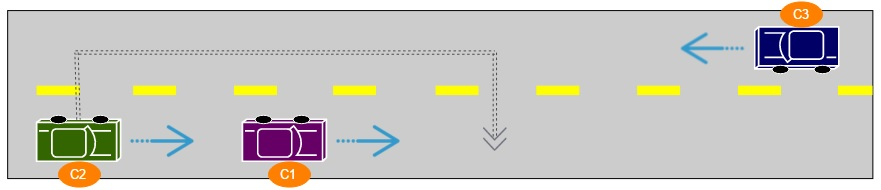
\includegraphics[width=400px, scale=1]{figuras/caso1}
  \caption{Demonstração do Caso 1}
\label{fig:caso1}
\end{figure}

Procedimentos:

\begin{enumerate}
  \item O CIAC identificará a intenção de ultrapassagem do condutor do Carro
  C2 que acionará o sistema por completo, monitorando as seguintes situações:
  \begin{itemize}
    \item Acionamento da seta;
    \item Mudança na angulação do volante, utilizando o sensor de rotação PST-360;
    \item Mudança de faixa, utilizando a câmera AWS650;
    \item Quando a distância entre o Carro C2 e o Carro C1 diminuir, utilizando a
    câmera AWS650, o Lidar HDL-64E e o Radar ARS-30X.
  \end{itemize}

  \item Em seguida, o sistema irá verificar se há presença de algum automóvel
  trafegando na mesma via em sentido oposto, fazendo uso da câmera AWS650, do
  Lidar HDL-64E e do Radar ARS-30X;

  \item Havendo a presença de um automóvel, nesse caso o Carro C3, o CIAC identificará:
  \begin{itemize}
    \item Posição geográfica do Carro C3, por meio da utilização do GPS
    A2100-A/B, do Radar ARS-30X e do Lidar HDL-64E;

    \item Velocidade do Carro C3, empregando o par Tranponder-Velocímetro do
    veículo, o Radar ARS-30X e o Lidar HDL-64E.
    \begin{itemize}
      \item Quando o CIAC identificar a intenção do condutor de realizar uma
      ultrapassagem, o transponder emitirá um sinal “questionador” do Carro C2
      para o Carro C3, solicitando, através da emissão de radiofrequência, a
      posição geográfica e a velocidade do Carro C3, dados que serão fornecidos
      pelo GPS e velocímetro do carro, respectivamente;

      \item E simultaneamente, a velocidade do Carro C3, a distância entre os
      carros C2 e C3 e tempo de encontro entre os mesmos estarão sendo aferidos
      com o auxílio do Radar, o qual emite ondas de rádio do Carro C2 que serão
      refletidas pelo Carro C3 e baseado no tempo de ida e volta do sinal
      obtêm-se a distância entre os dois carros, a velocidade do Carro C3 e
      assim, o tempo de encontro do Carro C2 com o Carro C3;

      \item E o Lidar, dispositivos que funciona com a emissão de um laser do
      Carro C2 que será refletido pelo Carro C3 e através do tempo de ida e
      volta desses pulsos é calculada a distância entre os carros C2 e C3.

    \end{itemize}
  \end{itemize}
\end{enumerate}
